% !Mode:: "TeX:UTF-8"
% !TEX program  = xelatex
\documentclass{sdureport}

% no head line or foot line
%\pagestyle{empty}

% just for filling a few pages
\usepackage{blindtext}
\usepackage{ctex}
\usepackage{indentfirst}
\usepackage{booktabs}
\usepackage{amsmath}
\usepackage{anyfontsize} % 公式字体报错问题
% initialize the variable texts
\sduCollege{计算机科学与技术}
\sduCourse{计算机组成与设计}
\sduSdudentId{202012345678}
\sduName{你的姓名}
\sduClass{你的班级}
\sduExperimentalTopics{实验2\  逻辑运算电路}
\sduExexperimentalHours{2h}
\sduDate{\today}

\begin{document}
\begin{sduDocument}
	\section{实验目的:}
	设计一个能实现1位逻辑乘$ab$、逻辑或$a+b$、半加$(a\bigoplus b)$的逻辑运算电路。

	\section{实验软件和硬件环境:}
	\begin{itemize}[leftmargin=1em]
		\item QuartusII 软件
		\item Windows10 Intel(R) Core(TM) i7-8750H CPU @ 2.20GHz
	\end{itemize}


	\section{实验步骤:}
	段落	段落	段落	段落	段落	段落
	段落



	段落	段落
	\subsection{二级标题}
	\subsubsection{三级标题}

	有序列表
	\begin{enumerate}
		\item 迭代次数:1868
		\item $\theta$:[-0.0566, 1.4720, 1.5706]
		\item 见:图\ref{L1}
		\item 见:图\ref{b1}
		\item 此学生不被录取的概率:0.6680
	\end{enumerate}

	\begin{figure}[H]
		\subfigure[Loss 变化曲线]{
			\label{L1}
			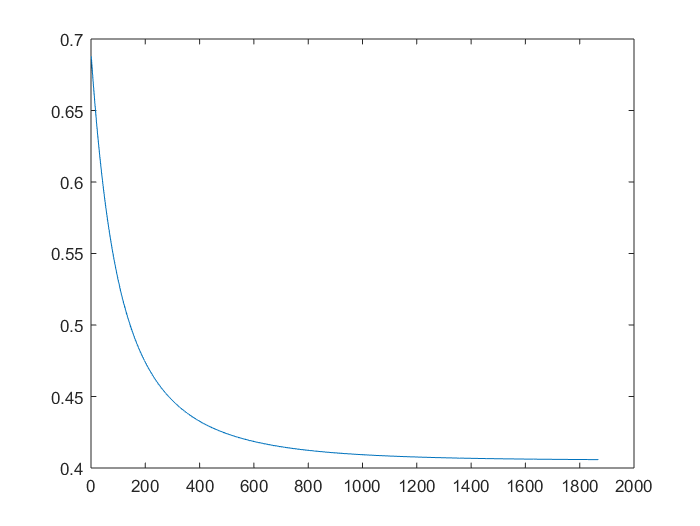
\includegraphics[width=0.45\textwidth]{figures/L1.png}}
		\subfigure[Decision Boundary]{
			\label{b1}
			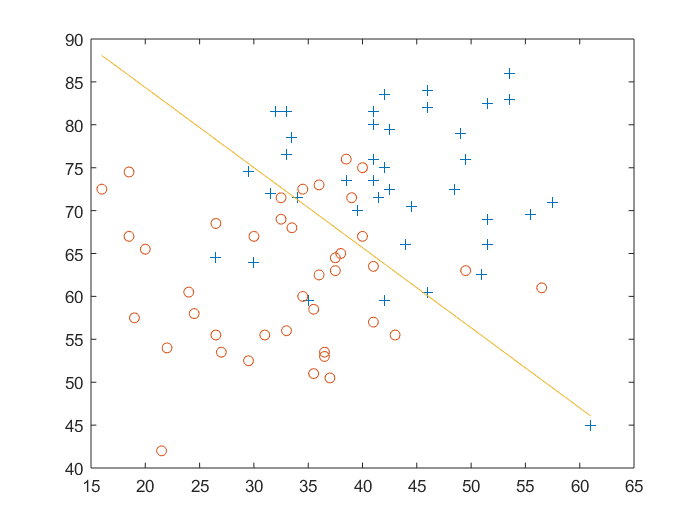
\includegraphics[width=0.45\textwidth]{figures/b1.png}}
		\caption{梯度下降法}
	\end{figure}
	\begin{figure}[H]
		\subfigure[Loss 变化曲线]{
			\label{L2}
			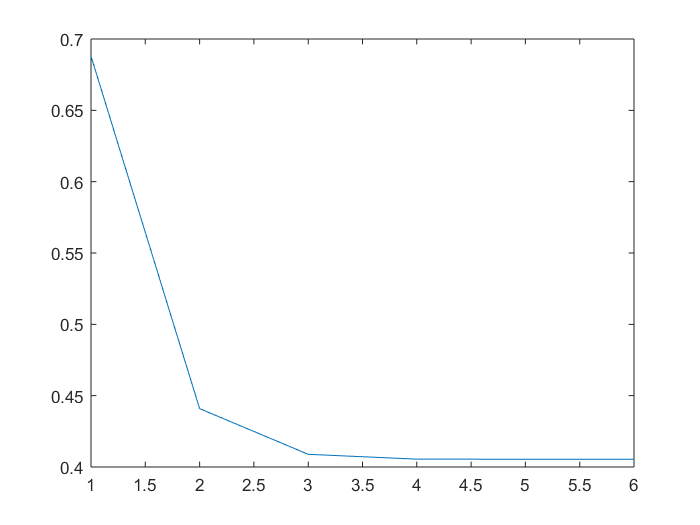
\includegraphics[width=0.45\textwidth]{figures/L2.png}}
		\subfigure[Decision Boundary]{
			\label{b2}
			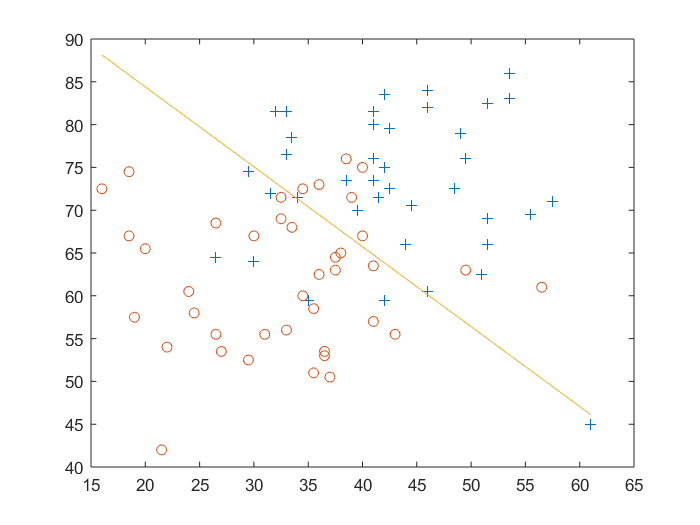
\includegraphics[width=0.45\textwidth]{figures/b2.png}}
		\caption{牛顿法}
	\end{figure}

\end{sduDocument}

\sduAppendix % 不需要附录二字注释掉这一行即可
\begin{lstlisting}[language=matlab]
	x = load("data2/ex2x.dat");
	y = load("data2/ex2y.dat");
	n = length(x);
	x = [ones(n, 1), x];
	stds = std(x);
	mu = mean(x);
	x(:, 2) = (x(:, 2) - mu(2)) ./ stds(2);
	x(:, 3) = (x(:, 3) - mu(3)) ./ stds(3);
\end{lstlisting}

\end{document}
